% Chapter Template

\chapter{Implementation} % Main chapter title

\label{Chapter5} % Change X to a consecutive number; for referencing this chapter elsewhere, use \ref{ChapterX}

\lhead{Chapter 5. \emph{Implementation}} % Change X to a consecutive
% number; this is for the header on each page - perhaps a shortened title

%----------------------------------------------------------------------------------------
%	SECTION 1
%---------------------------------------------------------------------------------------- 
\section{Integrate Henshin with DPF}
\label{integrate_henshin}

DPF is a framework where a domain specific modeling language can be defined over
several layers of abstractions. A specification 
$\spec{S}$\textsubscript{n+1} defines the abstract syntax for a specification
$\spec{S}$\textsubscript{n} at some abstraction layer.
The semantic behavior for a DPF specification $\spec{S}$\textsubscript{n} is
defined through model transformations that can specify different changes done to
the specification. There are already a natural
model transformation provided in DPF, and that is when a new specification is
created by the DPF Model Editor. A graph homomorphism is specified between
modeling elements in the newly created specification and modeling elements
provided one abstraction layer higher. In section~\ref{sec:abstraction_layer}
we described some model transformation examples according to different
abstraction layers. DPF does not provide support for an exogenous model
transformation that translates a specification described in one domain specific modeling language
to a model expressed in another domain specific modeling language. A new
specification will always be specified by a modeling language that corresponds
to a modeling formalism $\spec{S}$\textsubscript{n+1} one abstraction layer
higher. These specification may either be a user created specification or the
default specification provided by the framework.

\begin{figure}[H]
	\centering
	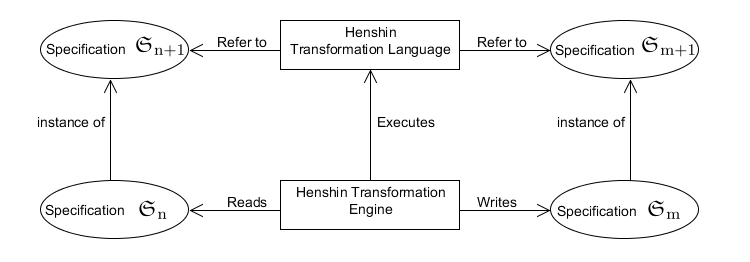
\includegraphics[scale=0.7]{./Figures/TransformationSolutionBasic.png}
	\caption[Integrating Henshin with DPF]
	{Using Henshin transformation language to translate a specification
	$\spec{S}$\textsubscript{n}.}
	\label{fig:Simple_Solution}
\end{figure}


Figure~\ref{fig:Simple_Solution} explains at top level how we want to integrate
the Henshin model transformation language with the Diagram Predicate Framework. Henshin
provides a transformation language and a transformation engine. We
use the Henshin transformation engine to read an instance specification
$\spec{S}$\textsubscript{n} and write an instance specification
$\spec{S}$\textsubscript{m}. To achieve this the transformation engine executes
a set of transformation rules written in the Henshin Transformation Language.
These transformation rules refers to the abstract syntax that is specified in
the modeling formalism $\spec{S}$\textsubscript{n+1} and the modeling formalism
$\spec{S}$\textsubscript{m+1} that the source and target model conforms to. 


\begin{figure}[H]
	\centering
	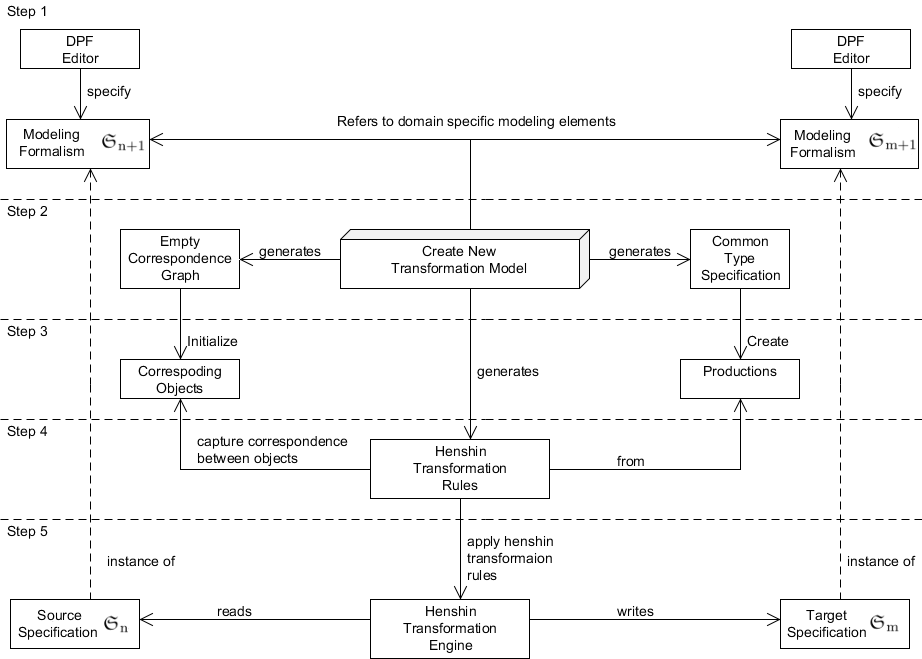
\includegraphics[scale=0.65]{./Figures/flowchart_v2.png}
	\caption[Work flow for the solution]
	{Progressively workflow for the problem solution.}
	\label{fig:work_flow_solution}
\end{figure}

Figure~\ref{fig:work_flow_solution} provides a diagram that is extended from the
previous figure~\ref{fig:Simple_Solution}. The diagram describes in five steps
how the editor progress from creation to execution of transformation rules. The
figure then explains that step 5 use the Henshin transformation engine that reads a
specification $\spec{S}$\textsubscript{n} and writes a specification
$\spec{S}$\textsubscript{m}. But before we can apply the actual transformation
we have to consider how the DPF Transformation Editor provides a set of Henshin
transformation rules.

\begin{enumerate}

\item At the first step we still have to provide a source modeling formalism
that contains a specification $\spec{S}$\textsubscript{n+1} and a target
modeling formalism that contains a specification $\spec{S}$\textsubscript{m+1}.
These specifications has an underlying graph that contains nodes and arrow that
represents the abstract syntax for the source and target specification. 

\item Step 2 consist of creating a new transformation model in the DPF
Transformation Editor. This new transformation model has references to a source
modeling formalism $\spec{S}$\textsubscript{n+1} and a target modeling formalism
$\spec{S}$\textsubscript{m+1}. With both the target and source modeling
formalism we create a $\spec{S}$\textsubscript{n+1} $\cup$
$\spec{S}$\textsubscript{m+1} specification that we use for typing
purposes for the transformation rules. An empty correspondence graph is also
generated.

\item Step 3 focus on creating the transformation rules through defining a set
of productions, where one production represents one transformation rule. A
single production specifies a LHS, RHS and an intersection graph that refer to
this common type specification,  $\spec{S}$\textsubscript{n+1} $\cup$
$\spec{S}$\textsubscript{m+1}. At the same time corresponding objects are
initialized by the user to specify the relation between source modeling elements
and target modeling elements. 

\item In step 4 we generate a set of Henshin Transformation Rules from these
productions and capture the correspondence between objects by specifying
traceable links.

\item In the final step we can apply these transformation rules to a Henshin
transformation engine and produce a target specification
$\spec{S}$\textsubscript{m}.

\end{enumerate}

One major challenge was processing Henshin transformation rules from modeling
elements that is represented in the source and target modeling formalisms.
These five steps describes the workflow of the DPF Transformation Editor. In
the next sections we will explore the most essential functionality of these
five steps and explain how we can integrate Henshin with the DPF workbench. But
first we will describe how a transformation rule is modelled in the Henshin
model transformation language.



%----------------------------------------------------------------------------------------
%	SECTION 2
%----------------------------------------------------------------------------------------

\section{Henshin meta-model}
\label{sec:henshin_meta}

The Henshin transformation language provides a meta-model that is an EMF based
model and uses the Ecore meta-model for typing purposes\cite{Arendt2010}. Since
this model is created based on EMF we know that EMF will generate interfaces and
a factory that we can utilize to implement Henshin transformation rules in Java.
We can specify a pattern graph and a replacement graph for each transformation
rule based on the factory class that the Henshin API provides. In the following
we will address what elements a transformation rule consist of based on
the Henshin meta-model for a transformation rule represented in
figure~\ref{fig:Henshin_metamodel}. The figure is obteined from a paper that
Thorsten Arendt, Enrico Biermann, Stefan Jurack, Christian Krause, and Gabriele
Taentzer published in 2010 on the Henshin transformation language where they
provide the meta-model for defining a single transformation
rule\cite{Arendt2010}.

\begin{figure}[H]
	\centering
	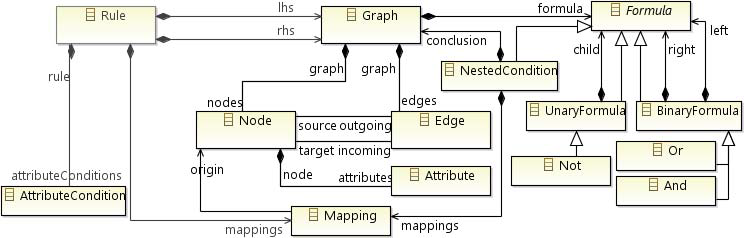
\includegraphics[scale=0.8]{./Figures/Henshin_metamodel.png}
	\caption[Henshin meta-model for a transformation rule]
	{Henshin meta-model for a transformation rule.}
	\label{fig:Henshin_metamodel}
\end{figure}

A \textbf{Rule} in Henshin represents a transformation rule that has a name,
a description and three properties. The first property disables or enables the
transformation rule, while the two other properties lets the user enable or
disable injective matching and the check dangling condition. The rule class
works as the root for all other modeling elements that are represented in 
figure~\ref{fig:Henshin_metamodel}. A new rule defines a left hand side and a
right hand side \textbf{Graph}. The LHS and RHS graph is formed by
creating nodes and edges. Nodes refers to objects in an instance graph and
edges refer to references between objects. An edge has a source and a target
node, while a node can have a collection of incoming and outgoing edges. The
nodes can also have a set of attributes attached. Nodes, edges and attributes
all have two common properties, and the first one is that they all have a type.

\begin{figure}[H]
	\centering
	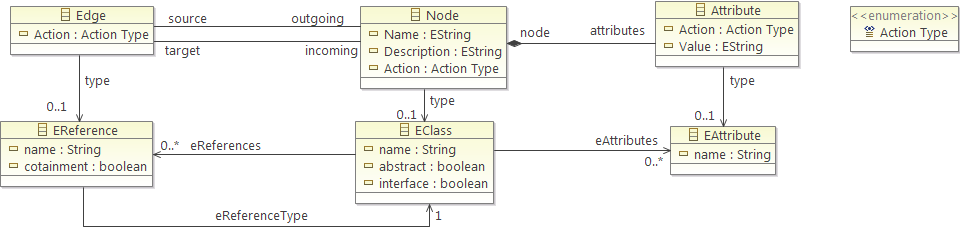
\includegraphics[scale=0.60]{./Figures/Node_edge_attribute.png}
	\caption[Henshin relationship with Ecore]
	{A simplified subset of the Ecore meta-model.}
	\label{fig:henshin_ecore}
\end{figure}

Figure~\ref{fig:henshin_ecore} represents a small fraction of the Ecore
meta-model and how Henshin modeling elements are typed by either an EClass,
EReference or EAttribute. For example a Node that is typed by a specific EClass
will only be matched to objects of this type in an instance model. These nodes
and edges are represented under a graph and form a pattern. Together with the
LHS and the RHS these patterns is either used to find matching patterns in a
source model or to create the corresponding pattern for a target model. The
second property that these three have in common is that they have an action
type. Action types are predefined stereotypes for Henshin that specifies the
semantics of a transformation rule. An action type could specify if a graph
modeling element is part of an application condition, the RHS, the LHS or an
intersection graph. A \textbf{Mapping} specifies how Henshin defines the
intersection graph. This is Henshin modeling elements that should be included
in both the LHS and the RHS graph. This means that these ojects should be part
of the matching pattern, but should not be deleted. A mapping has two
properties, namely an origin and an image. The origin property refers to a
given node from the LHS graph, while the image property specify a mapping to a
node in the RHS graph.

A rule can also specify a \textbf{Formula}, that determines restrictions for
match searching for a specific rule. A Formula modeling element is a child
of a graph and defines an application condition in Henshin. This formula class
can either be defined as an u-nary logical operation, a binary logical operation
or a nested condition. The first logical operation operates on a single operand
while the second operates on two operands, where these operands are represented
as a conditional statement that is either true or false. A rule can be applied
to an instance model if and only if all application conditions are valid. We
can basically have an unlimited nested formulas in Henshin, since a binary
formula can have a right and a left \textbf{Formula}, that again can be a
binary formula. Henshin however is only concerned whether this formula is valid
or invalid when a specific transformation rule is applied. A nested condition
provides a graph and a set of mappings to modeling elements that are part of
the LHS or intersection graph. This graph is a child of a nested condition and
contains nodes, edges and attributes that form a structural pattern that
specifies the application condition. We can observe that transformation rules
can have several number of application conditions. A binary formula can be of
type \textbf{Or} or \textbf{And} and provides the possibility to nest other
binary formulas. If the structure of a binary formula is the latter, then all
the application conditions in a binary formula has to be valid for a located
matching pattern.

\section{DPF Transformation Editor}

With the Eclipse Modeling Framework we created an Eclipse plugin where users can
create and modify transformation rules. Figure~\ref{fig:transform_metamodel}
provides the structural data model that we use to generate code for the model
implementation and the plugin implementation. The two classes Transform and
Production are the two domain classes that together defines this domain specific
modeling language that lets users create transformation rules. The Transform
class represent the DPF Transformation Editor and has a source meta-model and a
target meta-model, that corresponds to a source modeling formalism and a target
modeling formalism. The editor interprets a model transformation as endogenous
or exogenous if the target modeling formalism is equal or different to the
source modeling formalism. We also have the file location on the storage unit
for the source and target meta-model. The rules represents a collection of
transformation rules. These rules are typed by a Production that represent one
single transformation rule. A transformation rule has a name and contains a
graph that is stored internally for each rule.
This graph contains a pattern of nodes and arrows that the user can edit to
form a LHS graph, a RHS graph and an intersection graph. These graphs defines
several collections that contains nodes and arrows. These collections are
utilized by Henshin to generate transformation rules.

\begin{figure}[H]
	\centering
	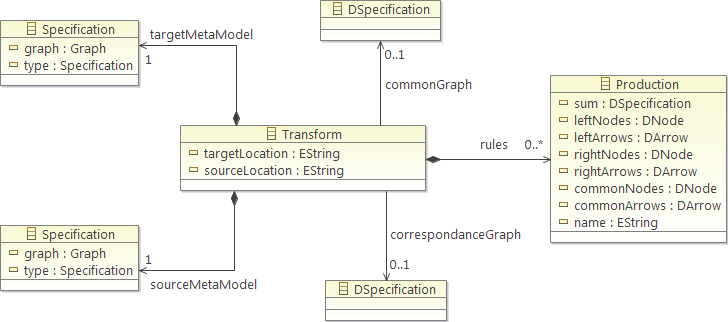
\includegraphics[scale=0.8]{./Figures/transform_metamodel_ecore.png}
	\caption[Model for the DPF Transformation Editor]
	{The domain model to create a DPF model transformation editor.}
	\label{fig:transform_metamodel}
\end{figure}

The user has to invoke the file creation wizard for the DPF Transformation Editor.
Other than choosing a project folder and a name for this new editor file, the
user has to specify what model is the source meta-model and what model is the
target meta-model. If the user do not specify a target meta-model then the file
creation wizard will interpret this as an endogenous model transformation.

The DPF Transformation Editor plugin has two editors that users can interact with.
The first is the master editor for the plugin and contains a list of the
transformation rules, where users can create, read, update and delete rules. The
second editor is administrated by the master editor, and each time a new
transformation rule is chosen, a simple version of the DPF Model Editor is
opened with a corresponding transformation rule. This editor is created from the 
Graphical Editing Framework (GEF) and is a graphical editor that includes a
toolbar. The toolbar is equal to the one used in  the DPF Model Editor and
contains modeling elements from the source and the target modeling formalism.

\begin{figure}[H]
	\centering
	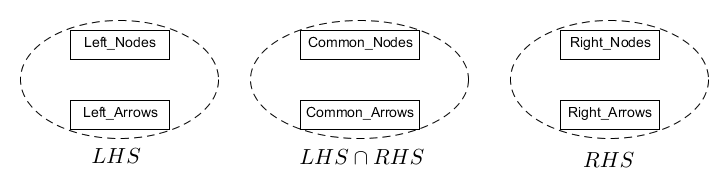
\includegraphics[scale=0.7]{./Figures/left_common_right.png}
	\caption[The three subgraphs for a transformation rule.]
	{Three subgraphs for each transformation rule in the editor.}
	\label{fig:lists_editor}
\end{figure}

The nodes and arrows from a source and target meta-model are used to create the
internal graph for each corresponding rule and uniquely map nodes and arrows to
three subgraphs represented as lists.
Figure~\ref{fig:lists_editor} represents the left, right and common subgraphs,
where each corresponding subgraph has a list of nodes and arrows. Each subgraph
represents a different part of a transformation rule according to graph
transformation. The left subgraph represents the LHS graph of a rule, while the
right subgraph represents the RHS graph. The common subgraph represents the
intersection between the pattern graph and the replacement graph. It is vital
for the model transformation to work that all the nodes and arrows are mapped
to one of these three subgraphs. This is entirely up to the user, because the
nodes and arrows from the LHS graph have to be created in such a way that the graph
can be matched in an instance graph.

Now that a list of transformation rules has been specified the user has to
initialise the model transformation environment. This is done through three
steps. 

\begin{enumerate}

\item \textbf{Generate Correspondence Graph.} The user has to
initialise a graph that contains the correspondence between objects. This is
important since Henshin cannot envision how modeling elements from a source
model are related to modeling elements from a target model. This relation has
to be specified prior to generating Henshin transformation rules. 

\item \textbf{Generate Henshin Rules.} Before we can use the Henshin model
transformation language we have to provide a module that contains a set of
transformation rules. And to achieve this we have to translate our
transformation rules that we defined in the editor into Henshin executable
rules.

\item \textbf{Apply Model Transformation.} By invoking the Henshin interpreter a
target model can be produced by applying a set of transformation rules to a
source model. The translated modeling elements can be assigned explicitly
to a corresponding target modeling formalism after a model transformation is
applied.

\end{enumerate}


\section{Generate Models}

Two models are required to be generated before a set of transformation rules can
be defined. These models are generated when a new model transformation is
initialised for the DPF Transformation Editor. Each of these two models has a
specific purpose for this integration of Henshin with the DPF Transformation
Editor. The first DPF specification that is generated combines modeling elements
from both the source and target modeling formalism while the second DPF specification
specifies a correspondence between source modeling elements and target modeling
elements. The creation process of the two models is similar, however the two
models are created differently. Figure~\ref{fig:Solution_CorrespondanceObjects}
illustrates how the two models are generated. 

\begin{figure}[H]
	\centering
	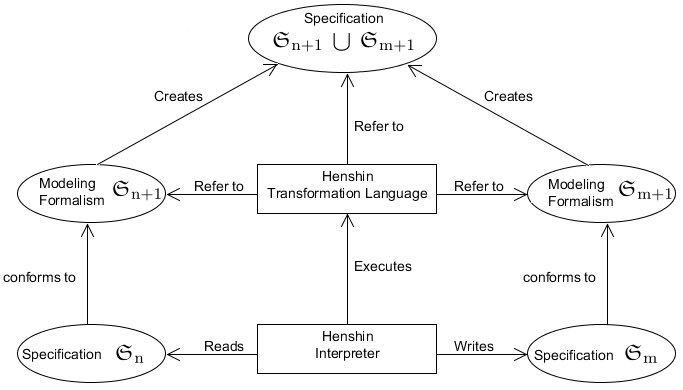
\includegraphics[scale=0.7]{./Figures/TransformationSolution_Correspond.png}
	\caption[Combination of a source and target modeling formalism]
	{Combination of a source and target modeling formalism.}
	\label{fig:Solution_CorrespondanceObjects}
\end{figure}

\subsection{Modeling Elements for Application Conditions}
\label{sec:modeling_elements}

This model is primarily used to create modeling elements for a production in the
DPF Transformation Editor. The integrated view to creating transformation rules
that the editor provides refers to this model for all created modeling elements.
We generate this model based on the specifications
$\spec{S}$\textsubscript{n+1} and $\spec{S}$\textsubscript{m+1} that are
provided by the corresponding modeling formalisms. A traceable link modeling
element is also specified and provides a source reference to source modeling
elements and a target reference to target modeling elements. A traceable link is
especially necessary if there is defined several nodes for a rule of the same
modeling element. This DPF specification is then referred to when a set of
productions are created according to the Henshin transformation language. An
application condition is specified for every occurrence of a node or an arrow in
a production. This is required for a Henshin rule to be able to include a
modeling formalism in a search pattern.

\subsection{Correspondence Graph}
The Henshin transformation language refers to modeling elements from a source
specification and a target specification when creating transformation rules.
However, the Henshin transformation language is unable to figure out how source
modeling elements are related to target modeling elements unless this is
provided explicitly. We can create a new DPF model that presents all the nodes
and arrows from the source specification $\spec{S}$\textsubscript{n+1} and
the target specification $\spec{S}$\textsubscript{m+1} as nodes. We then provide
a new modeling element that represents a bridge element between a source and a
target modeling element. We can specify an arbitrary number of these
modeling elements that binds nodes and arrows from a source model to nodes and
arrows from a target model. This DPF model specify the correspondence graph
between objects of a source and target meta-models. We can now refer to this
DPF model when creating Henshin transformation rules to extract the
corresponding objects. We use this correspondence graph or the trace object
that we mention in section~\ref{sec:modeling_elements} to determine how we
translate a source DPF specification. We create a trace object that has a
source reference to every matching node and arrow that the transformation
engine can locate and a target reference to the created nodes and arrows. In the
next section these traceable links are considered in more detail together
with how we generate a set of Henshin transformation rules.

\section{Generate Henshin Rules}
\label{hensin_rules}

We utilize the meta-model represented in figure~\ref{fig:Henshin_metamodel} to
create transformation rules in Henshin. We start with creating the root element
that is required for a Henshin model transformation and import EPackages that
is needed to define the content of a transformation rule. We need to import two
models if we want to translate a specification with Henshin. The first model is
the corresponding language syntax for all DPF specifications and the second
model is the meta-model for including traceable links in Henshin. We will describe the
purpose of these traceable links in more detail in subsection~\ref{Trace}. The
transformation language requires models that defines the abstract syntax for an
instance model to be able to specify modeling elements for both the LHS graph
and the RHS graph of a transformation rule. We can use meta-elements provided
by these two models when defining new nodes, edges and attributes in Henshin.
These types are created accordingly to the Ecore meta-model, and are EClass for
nodes, EReference for edges and EAttribute for attributes.

For Henshin we create one rule for each production provided by the DPF Model
Editor, where the name of the rule is acquired from the production. Henshin
provides a LHS, a RHS graph and a collection of mappings for each rule. We can
create a graph structure for the LHS and the RHS based on subgraphs that each
production provides. Modeling elements that form a pattern in the LHS are used
to find a match in a source model, while modeling elements that form a pattern
in the RHS are used to create new elements or replace these elements. Henshin
also include an intersection graph for each rule. This graph is not represented
as a physical graph like the LHS and the RHS are, but is represented as an
underlying graph that is formed based on these two graphs. The intersection
graph is represented by having elements in both the LHS and the RHS graph with mappings
that distinguish that these elements are one and the same. Now we have the LHS
graph, the RHS graph and the intersection of these two graphs that was
mentioned in section~\ref{sec:graph_based}. In this section we introduced double
and single pushouts of graphs. Henshin has an arbitrary mixing of these graph
transformation styles.

For each rule we created in the DPF Transformation Editor we have defined a
pattern, that either corresponds to a left hand side, a right hand side or a
common graph. This pattern consist of nodes and arrows that together form a
graph. For each node and arrow, we create a Henshin node that is either typed
as a Node or as an Arrow. An Arrow has to be represented as a Henshin node since
it is defined in the meta-model for a specification as an EClass. Now we have to
connect Henshin nodes with edges. An edge has three parameters, namely source,
target and reference. In Henshin we create an edge with a source Henshin node
and a target Henshin node. How the reference is typed depends on how the
source and target node refer to each other in the specification meta-model.
Figure~\ref{fig:arrow_node_relate} explains a simple example on how
the relationship between a node and an arrow are handled for a specification.

\begin{figure}[H] 
	\centering
	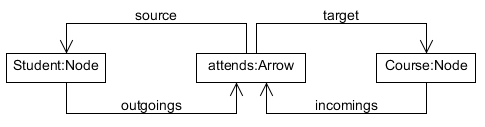
\includegraphics[scale=0.8]{./Figures/arrow_node_relate.png}
	\caption[Relationship between node and arrow in DPF]
	{Example of how nodes and arrows are related for a specification.}
	\label{fig:arrow_node_relate}
\end{figure}

An arrow that has a target and a source node, while every node has a list
of both incoming and outgoing arrows. So this means that a Node and an Arrow have a
similar relation in DPF models, where source and outgoings references represents
the same relation but are typed differently. It is however easier to coupe with
the arrows when creating transformation rules, since an arrow has an
one-to-one relationship, with a source node and a target node. How the typing
for an edge in Henshin is specified depends on the Henshin source and target
node. These nodes are typed by a corresponding EClass type from the
specification meta-model, that is a Node or an Arrow. An edge in Henshin can
specify a relation between two other Henshin nodes depending on how references
between Node and Arrow are typed. According to
figure~\ref{fig:arrow_node_relate} we have two references between arrow and
node and two references between node and arrow. If the source Henshin node for
an edge is typed by Arrow then the available references are source and target.
On the other side if the source Henshin node is typed by Node then we have a
zero to many relationship in the two references incomings and outgoings. When we
define relationships between two Henshin nodes we use the source and target
reference. This is because this is an one to one relationship between two nodes
and therefore we can always find the source and target node for a given arrow.
This means for every Henshin node that are typed by Arrow we have to specify two
relationships for this Henshin node. This is done by creating two edges in
Henshin, where one refer to source node while the other edge refer to
target node. This is achieved by specifying the Henshin node that is typed by
Arrow as source for both edges and switch between source and target as reference
for each target Henshin node. 

At this moment the pattern on the left hand side and the right hand side
are not specified by any types. The pattern conforms to the language syntax of
DPF models, however this is the case for all specifications regardless of
abstraction layer. A DPF specification is an instance of another
specification, and this is where we can retrieve the types for every node and
arrow. In the specification meta-model both the Node and Arrow class has a
reference type to another Node and Arrow. Figure~\ref{fig:pac_henshin}
represent how we want to employ application conditions in our Henshin rules to
locate a matching pattern in a source specification
$\spec{S}$\textsubscript{n}. Note that this figure represents a graph
structure for a specification that is composed of nodes and arrows that include
references to type nodes and arrows from the modeling formalism
$\spec{S}$\textsubscript{n+1}. This figure does not represent a LHS of a
transformation rule, but visualise how we want to locate matching modeling
elements in a source $\spec{S}$\textsubscript{n} based on a type node or a type
arrow. The idea is to create an application condition for every node and arrow
with their corresponding type node and type arrow. The node and arrow represents
the matching pattern in a specification $\spec{S}$\textsubscript{n} while the
reference to a type node and a type arrow is how the Henshin transformation
language can refer to the abstract syntax that the modeling formalism
$\spec{S}$\textsubscript{n+1} provides in DPF. The type nodes and arrows have
an attribute called name that can be used to specify a positive application
condition for a rule in Henshin. Positive application conditions are required
to be valid when searching through a source model for a transformation rule to
be applied.

\begin{figure}[H] 
	\centering
	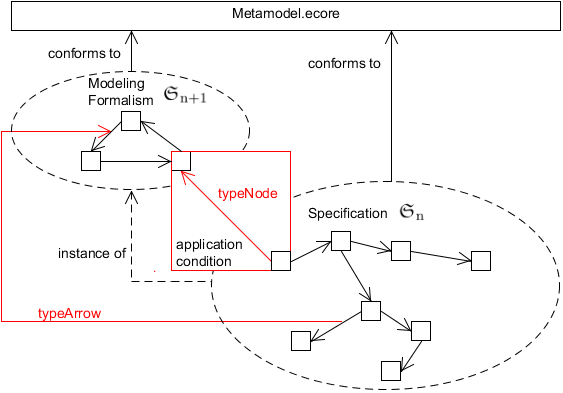
\includegraphics[scale=0.7]{./Figures/metamodelSpecification_PAC_1.png}
	\caption[How we want to handled types for a DPF model]
	{How we want to handle the abstract syntax one abstraction layer higher in
	the Henshin rules.}
	\label{fig:pac_henshin}
\end{figure}

This also leads to an important change in our Henshin rules, because we have to
include one more node and edge for every node and arrow. We have to create a new
Henshin node that represent the type node and type arrow and an edge that define
that this Henshin node is typed by another Henshin node. This is because when
Henshin is locating matches in an instance graph we want the transformation
language to locate matches for nodes or arrows that are typed by a specific
node or arrow from a modeling formalism one abstraction layer higher.
Figure~\ref{fig:pac_henshin_condition} explains how we solve this in Henshin.
We have a pattern graph or LHS on the right and an application condition graph
on the left. This specific transformation rule in Henshin specifies a simple LHS graph
that has an Arrow1 modeling element with a source Node1 and target Node2
elements. Note that the Arrow1 element is represented as a node and not as
an arrow like the graph structures in figure~\ref{fig:pac_henshin}. The reason
for this is because an arrow is represented as an EClass in the linguistic
meta-model for all specifications. Note that this LHS represents the graph
structure that is used to locate matching patterns in a source model. For this
example we want to locate all matching graph structures in a source
specification $\spec{S}$\textsubscript{n} that has an arrow with a
corresponding source node and target node. At the same time we specify
application conditions for this graph structure that correspond to a specific
typeNode and typeArrow. For this example we focus on the Node1 modeling
element.

\begin{figure}[H] 
	\centering
	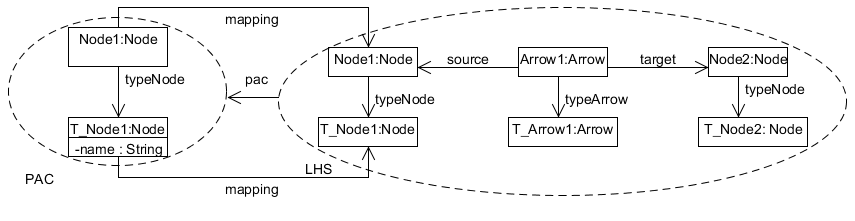
\includegraphics[scale=0.7]{./Figures/PAC_to_Henshin.png}
	\caption[How to handle node types for a rule in Henshin]
	{Defining a transformation rule that includes modeling elements from a
	specification one abstraction layer higher.}
	\label{fig:pac_henshin_condition}
\end{figure}

We discussed in section~\ref{sec:henshin_meta} that an application condition is
represented as a Formula in Henshin, and to solve typing of nodes and arrows in
DPF we need to create this Formula as a nested condition. This is because a
nested condition provides a set of mappings and a graph, where we can define
nodes, edges and attributes. To be able to map Henshin nodes is essential for
creating an application condition. We need to make sure that an application
condition is applied to a corresponding matched modeling element for a source
model. This is achieved by mapping Henshin nodes that are part of the graph in a
nested condition to Henshin nodes that are part of the graph pattern that
is used to locate matches. If we refer back to
figure~\ref{fig:pac_henshin_condition} we can see that the pattern graph has a
Node1 that are typed by a T\textunderscore Node1. We then define a
nested condition that contains these two nodes and a mapping from nodes
in the application condition to the nodes in the LHS or intersection graph. Now
we need to specify what an application condition should restrict when searching
through matches, and this is the name attribute of the type node or arrow
modeling element. This application condition can either be a positive or
negative application condition. In this case we want the name attribute to be a
positive application conditions that returns true for every matching type
element located in a source model. We can specify several application
conditions for a rule, and it depends on the graph structure of the LHS graph.
We define a new application condition for each nodes and arrows that are part of
the LHS graph, since these modeling elements can form a directed graph and each
modeling element is typed by a modeling element from the source meta-model. All
of these application conditions has to be true for a located match to be a
valid match. Now we will explore how we also implement negative application
conditions for our model transformation environment with traceable links.

\subsection{Traceable links}
\label{Trace}

As we discussed in chapter 3.2.7 a traceable link works as a footprint when
executing a set of transformation rules. Henshin provides a traceable link
implementation through the Henshin Trace model. This is a simple meta-model for
defining traceable links and can be imported for any Henshin module. The Henshin
Trace model provides an unique traceable
link between a source modeling element and target modeling element. The source
and target modeling elements can be any classes that conforms to the Ecore
meta-model. We create a traceable link for every Henshin node we have included
for the LHS graph. The nodes in the LHS graph are the source modeling elements
for a Trace modeling element while nodes in the RHS graph are the target
modeling elements. Now we have an unique link between a matched node from the
LHS graph and a produced node for the RHS graph for every time a transformation
rule is applied. These traceable links are represented in the replacement graph
the first time that a connection between two nodes are initialised. This means
that the traceable links are actually translated when a transformation rule is
applied and stored in the translated graph. Next time we want to refer to
a traceable link between modeling elements where a transformation rule has been
applied we have to make sure that the trace object is created both in the LHS
and the RHS with a mapping between them. Because together with a negative
application condition this traceable link will make sure that we only translate
located matches in an source model once. This can be achieved by defining a
negative application condition that forbids Henshin to create a traceable link.
We create a nested condition similar to the previous section, but for this case
we want the application condition only to return true for all matches that does
not contain this graph pattern. This is very convenient when applying a set of
transformation rules, because we have already stated that a traceable link is
created when a transformation rule locates a match in an instance graph. This
means that we create unique traceable links between all nodes in the pattern
graph that is matched in an instance graph and the nodes that we create. It has
to be noticed that the source and target nodes of a traceable link has to be
typed by the EClass modeling element that Ecore provides. We can now execute
the set of transformation rules as long as we want and be safe that we will not
execute matching pattern in an instance graph more than once. The reason that
we can make this statement is because when we find a match for the first time
then there exist no traceable link to these modeling elements. But once the
transformation engine execute this rule, then a traceable link is initialised
between the matching nodes on the left side and the corresponding modeling
elements on the right side. Now the transformation engine cannot 
locate this specific match for a second time because we have restricted the
transformation rule to not include matches that has a traceable link to the
source node that are part of the LHS graph. Now we will describe more in detail
how we apply these transformation rules.

\section{Apply Model Transformation}

\subsection{Rule Application Control}

Now that the DPF Transformation Editor has generated a set of Henshin
transformation rules the transformation engine is ready to apply these rules to
a source model. The Henshin module we generated in the previous section now contains a set of
transformation rules that are defined accordingly to the the Henshin
transformation language. The Henshin Transformation Engine can now execute this
generated module by explicitly invoking the Henshin interpreter. The
interpreter requires a module, a graph that contains the source model and a
Henshin unit before it can be applied. For our solution we have created a
transformation unit that executes a set of transformation rules in the same
order that the DPF Transformation Editor provides, and is called a Sequential
unit. A transformation unit in Henshin is an implementation of a rule
application control system that we described in a more general term in section
3.2.3. A transformation unit in Henshin is an executable part that the
transformation engine can interpret and apply rules accordingly. It is
important to specify that a transformation rule itself in Henshin is a
transformation unit, and can therefore be executed by Henshin's transformation
engine. But a Henshin transformation rule does not provide any control
mechanism for it self or other rules when executed.
A transformation rule will therefore only locate one single match if we
invoke the Henshin interpreter on a single rule. This is one reason for why we want to
specify a transformation unit that has some unique properties that a single
transformation rule does not provide. Some Henshin transformation units have the
possibility to have other transformation units as subunits.
The Sequential unit that the module provides works as the master unit for
applying the transformation rules. For each transformation rule we created in
the previous section we define a Henshin Loop unit. This unit can only contain
one single subunit, and that is a corresponding transformation rule. The
Loop unit is executed for as long as there are any matching modeling elements
in an instance graph and will locate matches an unlimited number of times
unless we provide any mechanism to stop the unit. This is where the negative
application conditions that we described in the previous section plays a vital
role. Because the negative application condition specifies that a
transformation rule will only be applied unless there exist no traceable links.
The first time the transformation engine locates a match for a transformation
rule it will create a traceable links that connects the matching modeling
elements and the created modeling elements. Now the next time this specific
match is located the application condition will not be valid since now there
exist a traceable link that has a reference to a modeling element in the source
model. We can now apply these repeatable units for all transformation rules as
long as the input graph does not contain a traceable link for a matched
modeling element.

\subsection{The Transformed Model}

For all matches found in a source model we do some changes depending on how the
RHS graph is specified. These changes are specified as new DPF modeling elements
after applying a set of transformation rules. The next step is to make sure that
the produced modeling elements are type correct. This means that the target
model is required to conform to a target modeling formalism.
Figure~\ref{fig:transformed_model} represents the result of a model to model
transformation.

\begin{figure}[H] 
	\centering
	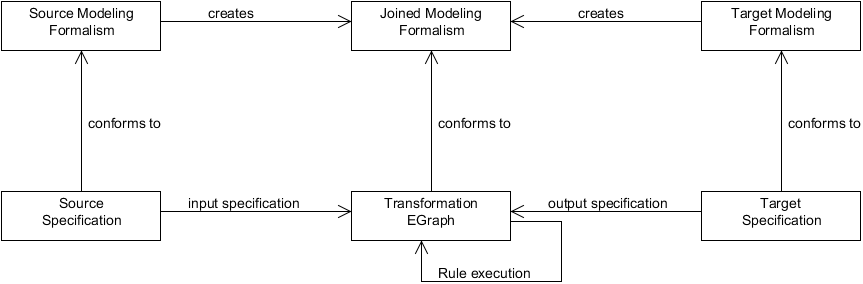
\includegraphics[scale=0.7]{./Figures/Transformed_model.png}
	\caption[The transformed specification]
	{The transformed result of a model to model transformation.}
	\label{fig:transformed_model}
\end{figure}

The transformation EGraph represents the source model as we mentioned in the
previous section. The Henshin interpreter will execute transformation rules on
this transformation graph until there are no more valid matching pattern located
in the source model. The produced target modeling elements that are included in
the transformation graph after rule execution conforms to a joined modeling
formalism. However, we want these modeling elements to conform to a target
modeling formalism and not the joined modeling formalism.
Section~\ref{hensin_rules} describes how we can create a set of transformation
rules in Henshin from the transformation rules in the DPF Transformation Editor.
These transformation rules has a search graph structure with positive
application conditions that determine the abstract syntax that a source
modeling formalism one abstraction layer higher provides. Each Henshin node in a
RHS graph of a rule that is specified has a reference to a target type node or
arrow. For each application of a transformation rule we locate a match and
create nodes and arrows with a corresponding type node and type arrow
accordingly to the RHS. After the execution of all the transformation rules we
can now extract these produced target modeling elements to a new target
specification that conforms to a target modeling formalism. For each translated
modeling element we can check if it has a corresponding type node or type arrow
in the target modeling formalism. 

\section{Solution summary}

So far we have extended the DPF Transformation Editor to support exogenous model
transformation between different abstraction layering hierarchies. In this
section we will summarize some of the features this solution provides.

\begin{itemize}
  	\item The DPF Transformation Editor provides an integrated view to define
	transformation rules. The different modeling elements that is created for a
	specific transformation rule can be mapped to either a left subgraph, a right
	subgraph or a common subgraph.
	
	\item Two DPF specifications are specified that the Henshin transformation language
	can utilize when creating transformation rules. One of the generated models
	specify the correspondence of objects and requires the user to define
	how a source modeling element relate to a target modeling element for a
	specific model transformation.
	
	\item The DPF Transformation Editor can invoke the Henshin interpreter to
	create a set of transformation rules according to the Henshin meta-model.
	
	\item A transformation rule in Henshin refers to the abstract syntax from
	a modeling formalism one abstraction layer higher by specifying an application
	condition for every occurrence of a modeling element in a transformation rule. 
	
	\item We create a traceable link that includes a matched source modeling
	element and a corresponding produced target modeling element. This traceable
	link is used to be certain that the transformation engine does not locate
	duplicate matches and if already translated target modeling elements are
	defined in other transformation rules.
	
	\item We invoke the Henshin interpreter programmatically to apply
	the set of Henshin transformation rules to a source specification.
	
	\item After the transformation we extract the produced modeling elements from
	the translated graph to a specification and explicitly specify that the
	modeling elements conforms to modeling elements of a target modeling formalism
	one abstraction layer higher.
   
\end{itemize}


